\documentclass[a4paper,12pt]{article} % Aumentato a 12pt per maggiore leggibilità

% Pacchetti fondamentali
\usepackage[utf8]{inputenc}
\usepackage[italian]{babel}
% Margini ottimizzati: più larghi ai lati (1cm) e più distribuiti in altezza (1.5cm)
\usepackage[top=1.5cm, bottom=1.5cm, left=1cm, right=1cm]{geometry} 
\usepackage{graphicx} 
\usepackage{nopageno} 
\usepackage{xcolor}
\usepackage{amsmath, amssymb} % Per le formule matematiche avanzate
\usepackage{fontawesome5} % Per le icone (telefono, email, ecc.)
\usepackage{tcolorbox} % Per creare riquadri colorati e accattivanti

% Definizione dei colori personalizzati
\definecolor{mainblue}{RGB}{45, 90, 150} 
\definecolor{accent}{RGB}{220, 80, 40}
\definecolor{lightgray}{RGB}{245, 245, 245}

\begin{document}

% --- INTESTAZIONE COLORATA ---
\begin{center}
    {\Huge \textbf{\faRocket\ FISICA E MATEMATICA}}\\[0.3cm]
    {\Large \textit{Lezioni private, recupero debiti e preparazione test}}
\end{center}
\vspace{0.4cm} 

% --- CORPO CENTRALE DIVISO IN DUE ---
\noindent
\begin{minipage}[t]{0.63\textwidth} % Leggermente più larga per dare più respiro al testo
    \vspace{0pt} % <-- TRUCCO: Forza l'allineamento in alto con l'altra minipage
    
    \textcolor{mainblue}{\Large \textbf{\faUserGraduate\ Chi sono}}\\[0.2cm]
    Mi chiamo \textbf{Nicolò Favagrossa}. Sono uno studente \textbf{Magistrale in Fisica} (specializzato in Particelle e Astroparticelle) con oltre due anni di esperienza professionale come \textbf{Tecnico di laboratorio R\&D Junior} nel settore energetico. \\
    Durante la mia triennale in \textbf{Fisica} all'\textbf{Università Statale di Milano} ho collaborato a esperimenti internazionali come JUNO (Jiangmen Underground Neutrino Observatory). \\
    \textbf{Il mio obiettivo} non è solo farti superare la verifica, ma trasmetterti la passione per la scienza. Voglio aiutarti a scoprire la logica che si nasconde dietro ogni problema, trasformando la fatica dello studio in pura curiosità!\\[0.4cm]
    
    \textcolor{mainblue}{\Large \textbf{\faChalkboardTeacher\ Cosa offro}}\\[0.2cm]
    \begin{itemize}
        \setlength{\itemsep}{0.25cm} % Aumenta lo spazio tra i punti dell'elenco sfruttando lo spazio sotto
        \item[\textcolor{accent}{\faCheckCircle}] \textbf{Recupero Debiti:} Hai il debito in Matematica o Fisica? Creiamo insieme un piano di studio estivo mirato per superare l'esame di riparazione a settembre con sicurezza e senza stress.
        \item[\textcolor{accent}{\faCheckCircle}] \textbf{Ripasso e Potenziamento:} Consolidamento delle basi, recupero delle lacune e preparazione per chi vuole iniziare il prossimo anno scolastico con una marcia in più.
        \item[\textcolor{accent}{\faCheckCircle}] \textbf{Test d'Ingresso:} Allenamento logico e preparazione specifica per superare i TOLC e i test di ammissione universitari.
        \item[\textcolor{accent}{\faCheckCircle}] \textbf{Zero Perdite di Tempo:} Ti chiedo di inviarmi gli argomenti prima di vederci. In questo modo preparo una lezione su misura, con schemi ed esercizi già pronti per sfruttare al 100\% il tempo.
        \item[\textcolor{accent}{\faCheckCircle}] \textbf{Online o in Presenza:} Massima flessibilità. Lezioni a distanza super interattive grazie all'uso di videocamera e tablet condiviso in tempo reale.
        \item[\textcolor{accent}{\faCheckCircle}] \textbf{Supporto SOS:} Ti blocchi su un esercizio a casa? I miei studenti possono scrivermi in qualsiasi momento per un aiuto veloce o un consiglio metodologico!
    \end{itemize}\vspace{0.4cm}
    
    \textcolor{mainblue}{\Large \textbf{\faAddressCard\ Contatti}}\\[0.2cm]
    \faPhoneSquare\ Telefono / WhatsApp: \textbf{389 0155686}\\
    \faEnvelope\ Email: \textbf{nicolo.favagrossa@gmail.com}
    
\end{minipage}%
\hfill
\begin{minipage}[t]{0.34\textwidth}
    \vspace{0pt} % <-- TRUCCO: Si allinea esattamente alla prima riga di "Chi sono"

    % --- IMMAGINE MODELLO STANDARD ---
    \begin{center}
        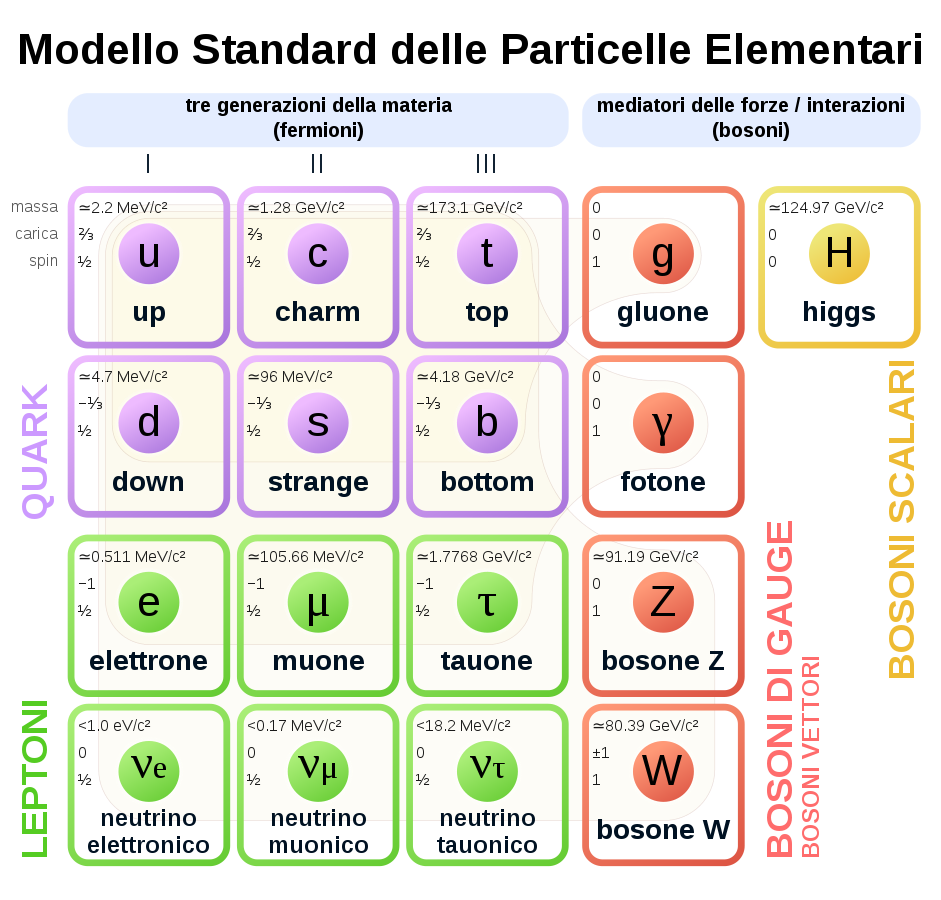
\includegraphics[width=1.07\textwidth, keepaspectratio]{Modello Standard.png}
        \vspace{0.4cm} 
    \end{center}

    % --- RIQUADRO ESTETICO DELLE FORMULE ---
    \begin{tcolorbox}[colback=lightgray, colframe=mainblue, arc=2mm, title=\faAtom\ \textit{L'Evoluzione della Fisica}, left=4pt, right=4pt, top=5pt, bottom=5pt, boxsep=2pt]
        \centering
        {\small \textbf{Meccanica Classica}}\\
        $F = ma$\\[0.2cm]
        {\small \textbf{Meccanica Analitica}}\\
        $\displaystyle \frac{d}{dt} \left( \frac{\partial \mathcal{L}}{\partial \dot{q}_i} \right) - \frac{\partial \mathcal{L}}{\partial q_i} = 0$\\[0.2cm]
        {\small \textbf{Meccanica Quantistica}}\\
        $\displaystyle i\hbar \frac{\partial \Psi}{\partial t} = \hat{H}\Psi$\\[0.2cm]
        {\small \textbf{Meccanica Quantistica relativistica}}\\
        $(i\gamma^\mu\partial_\mu - m)\psi = 0$\\[0.2cm]
        \rule{0.85\linewidth}{0.8pt}\\[0.15cm]
        \textit{\scriptsize Dalla semplicità alla complessità di una formulazione sempre più generale.}
    \end{tcolorbox}
    
    \vspace{0.4cm}
    
    \begin{center}
        % Spazio per QR Code 
        
\includegraphics[width=3.2cm]{qr.jpeg}\\[0.15cm]
        \small \faLinkedin\ \textit{Inquadra per il mio profilo!}
    \end{center}
\end{minipage}

\end{document}